Whole project is designed to be deployed in the cloud and in particular in KaaS(kubernetes as a service) solution. For comparison of most popular cloud providers, open-sourced cost calculator\cite{managed_kubernetes_pricing} was used. Result for most popular cloud provider: amazon web services(AWS), azure(AKS), google cloud(GKE) and digital ocean(DO) can be seen on plot below:

\begin{figure}[H]
    \centering
    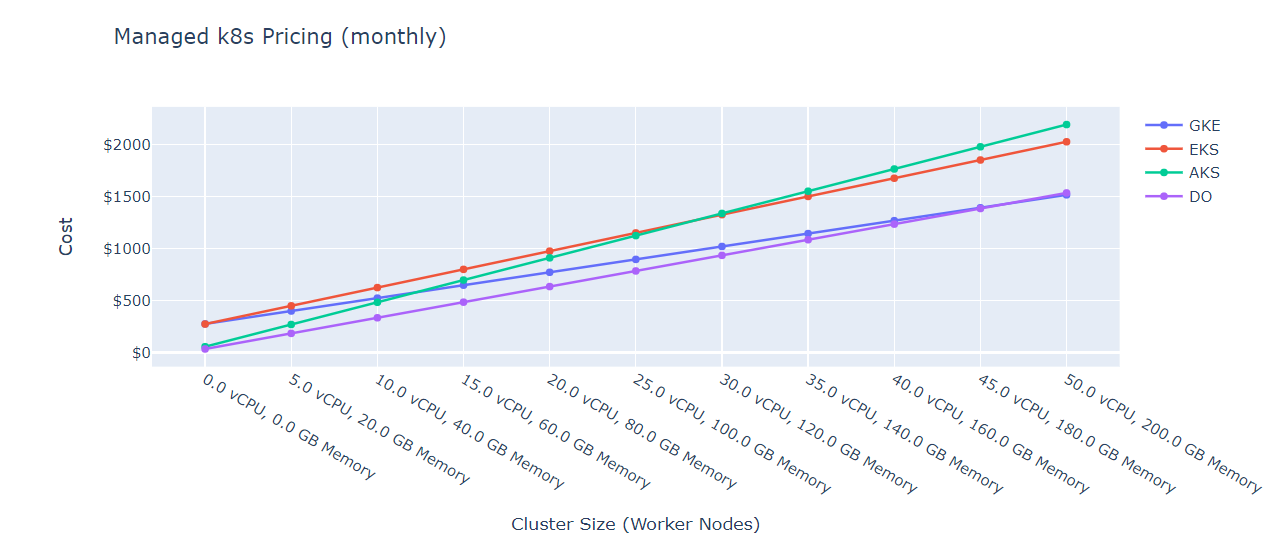
\includegraphics[width=01\textwidth]{pictures/k8s_cost.png}
    \caption{ Local development }
    \label{fig:k8s_cost}
\end{figure}

Cheapest options for small scale projects are digital ocean and azure because they doesn't charge for the compute used for the control plane. For large projects Google Cloud is the most affordable. 

Two cloud  providers were tested for this implementation: Microsoft azure and Okteto Cloud. Both are offering kubernetes as a service, but they have chosen different approaches. 

In azure kubernetes cluster is being created and then it is mostly managed by the user. It is harder to maintain but also more flexible as cluster can be scaled and extended easily.  

Okteto cloud has taken different approach, it is focused on crating development enviroment which is usually not production ready. In free tier they provide namescpace in a cluster(fully managed by okteto) with possibility to deploy up to 10 pods with limitations mentioned below:
\begin{itemize}
    \item Namespaces: 5
    \item Pods: 10
    \item CPU: 1 / pod
    \item Memory: 3Gi / pod
    \item Storage: 5Gi
\end{itemize}

Bottom line: Okteto for development azure for pruductization.